\begin{figure} [htb]
  \setlength{\unitlength}{\textwidth}

        \begin{picture}(1,0.46)(0,0.4)

      \put(0.1,0.45){\includegraphics[width=0.75\unitlength]{./chapter-cross-sections/fnp/qss-dns-mean-power.eps}}
      
%       \put(0.07,0.95){$\displaystyle\frac{V}{D}$}
%       \put(0.07,1.3){$\displaystyle\frac{A}{D}$}
       \put(0.06,0.68){$\displaystyle\frac{P_{m}}{\rho \mathcal{A}U^3 }$}
%       \put(0.5,0.4){$\massdamp$}
       \put(0.5,0.42){$\displaystyle\ratio$}
    
    \end{picture}

  % \caption{Comparison of maximum power between QSS and DNS data obtained using 3 point local quadratic curve fitting.The error was obtained using Eq:\ref{eqn:error_calculation}}
    \caption{Comparison of the maximum power obtained using DNS ($\displaystyle\bullet$) and the QSS ($\times$) model as a function of \ratio. Data obtained at $\massstiff=1000$ ($\mstar=201.3$) and $\reynoldsnumber=200$. Similar trends are present for both QSS and DNS data. A significant reduction in power could be observed as $\ratio \rightarrow 1$}
    \label{fig:DNS-power}
\end{figure}

 %vspace{10cm}